\subsection{Global History Buffer Prefetcher}
\label{sec:ghbPcdcPrefetcher}

The global history buffer prefetcher is an instruction based
prefetching scheme, i.e. a prefetcher which uses the value of the
program counter at the memory access time to gather statistics about,
and from these predict, future memory accesses for the given load. In
this scheme, a datastructure called Global History Buffer (abbreviated
GHB) is maintained. This datastructure is a table whose elements are
addresses for which a cache miss has recently occurred, as well as a
pointer to the previous table element representing a miss
corresponding to the same program counter as the given miss. The
structure is illustrated in figure~\ref{fig:ghbStruct}.

\begin{figure}[ht]
  \centering
  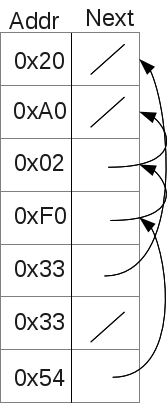
\includegraphics[scale=0.5]{figures/ghb_diag.png}
  \caption{\label{fig:ghbStruct} Structure of the GHB. Each table
    element contains two items: The requested address, and the
    previous cache miss from the same program counter as this entry
    came from.}
\end{figure}

Complementary to this table, an index table is used to record the last
entry inserted into the GHB for a given program counter value. With
these two datastructures, you can obtain the recent miss history for a
given load by traversing the linked list of table entries. There are
several ways to use this information to predict what addresses might
be needed in the future. We have decided to implement a version called
GHB/PCDC (Global History Buffer, Program Counter based with Delta
Correlation \cite{Grannas}). The idea is to extend the constant stride
prefetcher with the ability to recognize patterns of non-constant
stride accesses. Specifically, on a cache miss the offsets between
previous misses for the current program counter is computed and stored
in what is known as a delta table. An example of this is given in
figure~\ref{fig:deltaTableComp}. 

\begin{figure}[ht]
  \centering
  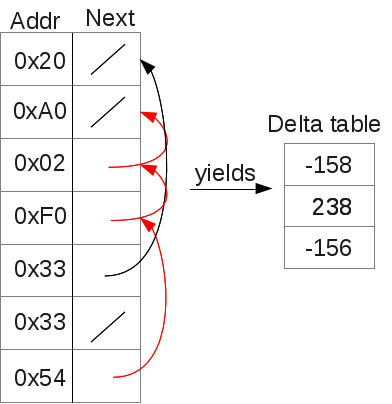
\includegraphics[scale=0.5]{figures/delta_table_comp.png}
  \caption{\label{fig:deltaTableComp} Computation of a delta table for
    a given miss, where the miss history is marked with red
    arrows. The four registered misses results in three delta values.}
\end{figure}

The delta table is then searched backwards for the previous occurrence
of the last two delta values. In our example in
figure~\ref{fig:deltaTableComp}, we would search for the delta values
238 and --156. If these have not occurred previous, as they indeed
have not in our example, then we do not prefetch anything as we have
no information about the past. If they are found, however, we prefetch
addresses according to the deltas which followed the previous delta
pair occurrence. 

An example of where this technique would improve upon the stride
prefetcher follows, as given in \cite{Nesbit}. Assume you access the
first few columns of each row of a multidimensional array. This would
result in a few constant stride misses, followed by a miss with a
delta corresponding to the size of the remaining row. A stride
prefetcher would issue prefetches for the constant stride, which would
be unneeded when you start accessing the next row.
% Furthermore, if the number of columns accessed was small the stride
% prefetcher might not register the constant stride in time to
% actually perform any useful prefetches
In contrast, the delta correlating prefetcher would create a history
buffer which paid heed to the larger delta value. On subsequent misses
to the next row, it would look up in its history table that what
follows this large delta is actually a series of constant stride
misses. It could then start prefetching sensible addresses right away.

Another example would be code which traverses the same linked data
structure multiple times. Consider the following loop:

\begin{lstlisting}
  void f(list *l) {
    for (list *n = l; n; n = n->next) {
      process(n);
    }
  }
\end{lstlisting}

In particular, consider the end-of-loop statement {\lstinline|n =  n->next|}. 
Assuming a register {\lstinline|r1|} contained {\lstinline|n|}, this
would compile into something like the following:
\begin{lstlisting}
  ld r1, [r1, nextOffset] @ 1. Load the offset value
  ld r1, [r1]             @ 2. Load the next pointer
\end{lstlisting}
The second statement would access addresses with a delta value of the
elements of the list. So would the first statement, as the offset of
the {\lstinline|next|} field is constant in the data structure. In
fact, so should most loads and stores accessing {\lstinline|n|} in
{\lstinline|process|}, given that they do not occur within nested
loops. The first time {\lstinline|f|} is run there would be no
benefit, but if it is a function that is called a lot with the same
list then on future calls the first iterations should register the
start of the loop, and prefetch the addresses belonging to elements
further on in the list.

{\bf (references, citations)}
